\documentclass[12pt, titlepage]{report}
\usepackage[spanish]{babel}
\usepackage[none]{hyphenat}
\usepackage[margin=3cm]{geometry}
\usepackage{graphicx}
\usepackage{subcaption}
\usepackage[hidelinks]{hyperref}
\usepackage{parskip}
\usepackage[shortlabels]{enumitem}
\usepackage{longtable}
\usepackage{multirow, makecell}

\sloppy
\setlength{\parindent}{0cm}
\graphicspath{{img/}}
\decimalpoint
\hypersetup{colorlinks=true, urlcolor=blue}
\urlstyle{same}

\begin{document}
    \begin{titlepage}
        \begin{center}
            \begin{figure}[ht]
                \centering
                \begin{subfigure}[r]{0.15\textwidth}
                    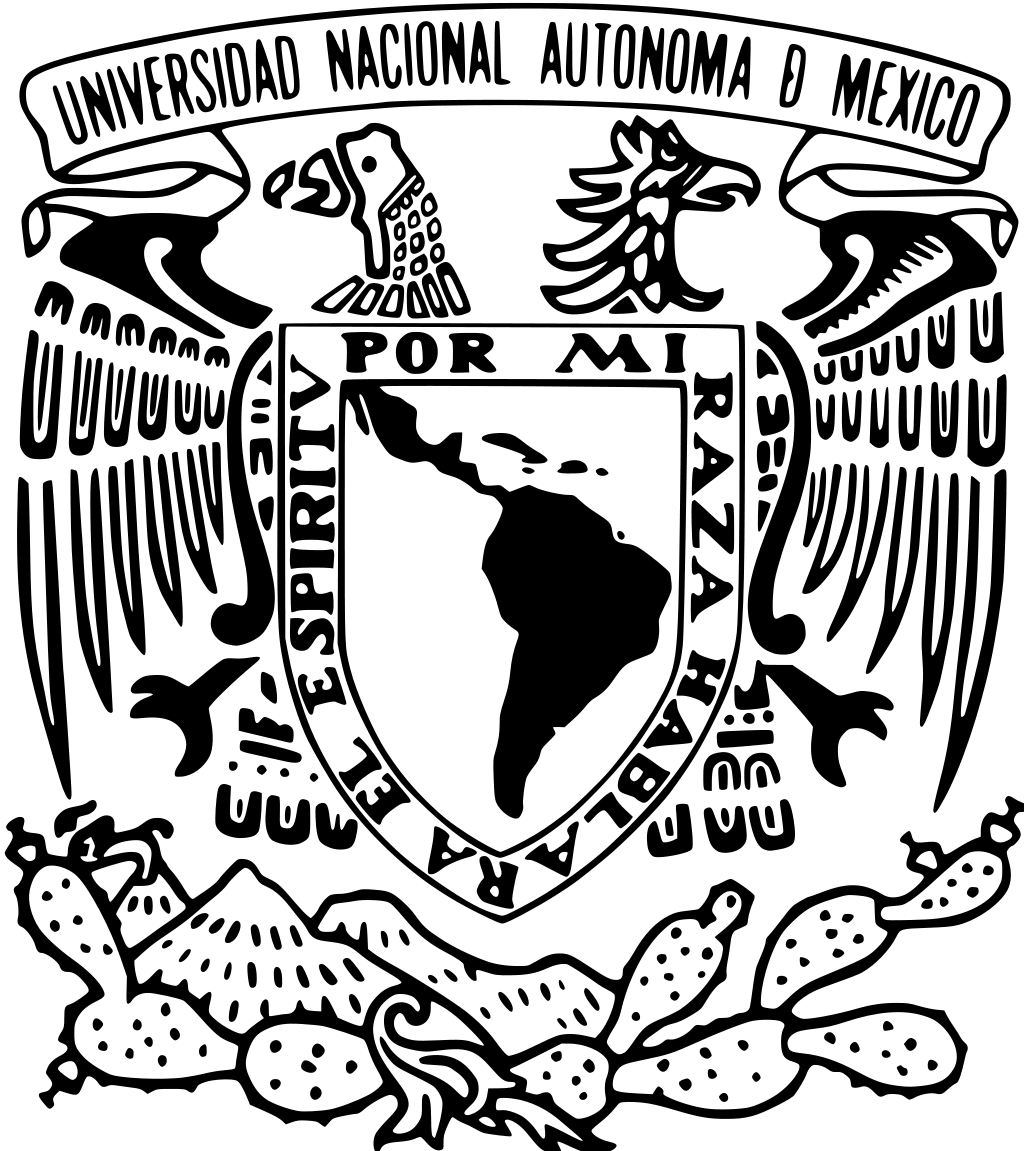
\includegraphics[width=\textwidth]{Escudo_UNAM.png} 
                \end{subfigure} \hspace{9cm} 
                \begin{subfigure}[l]{0.15\textwidth}
                    
\includegraphics[width=\textwidth]{Escudo_FI.png}
                \end{subfigure} 
            \end{figure}

            \large \textbf{UNIVERSIDAD NACIONAL AUTÓNOMA DE MÉXICO\\}
            \textbf{\\FACULTAD DE INGENIERÍA\\} 
            \hfill \break
            Laboratorio de Mecánica\\
            \Large \textbf{\\Práctica No. 5\\}
            \large Movimiento rectilíneo uniformemente variado\\
            \Large \textbf{\\Nombre del profesor\\}
            \large Lorenzo O. Miranda Cordero\\
            \Large \textbf{\\Grupo 8\\}
            \textbf{\\Brigada 4\\}
            \textbf{\\Integrantes:\\}
            Acosta Porcayo Alan Omar\\
            Bonilla López Mauricio Gael\\
            Cisneros Rojas Héctor Manuel\\
            Domínguez González Andrea\\
        \end{center}
        \begin{flushright}
            \Large \textbf{Semestre 2023-2}
        \end{flushright}
    \end{titlepage}

    \section*{Introducción}
    Se llama movimiento rectilíneo uniformemente variado a aquel movimiento rectilíneo de una partícula en el cual el valor de la aceleración es constante.

    Este tipo de movimiento se presenta en la caída libre, el tiro vertical y en el movimiento de cuerpos bajando por un plano inclinado.

    Es relativamente fácil de reproducir en el laboratorio, y es por ello que frecuentemente se le escoge para verificar el comportamiento cinemático de los cuerpos con dicho movimiento.

    La fuerza de fricción seca es una fuerza tangencial entre dos superficies que tiende a oponerse al movimiento relativo de dichas superficies.

    El comportamiento de esta fuerza lo establecen relaciones empíricas determinadas por las leyes de Coulomb-Morin, las cuales no constituyen leyes físicas científicas fundamentales como las leyes de Newton.

    El coeficiente de fricción cinética depende principalmente de la naturaleza de las superficies en contacto, es relativamente grande cuando son muy ásperas y pequeño cuando están razonablemente pulidas; además, varía algo con la velocidad relativa y es más o menos independiente del área en contacto, aunque para efectos prácticos se le considera invariante con respecto a la rapidez de movimiento.

    La determinación del coeficiente de fricción cinética de manera experimental es muy importante para la comprensión y el análisis de los fenómenos en los que se presenta. 

    \section*{Objetivos}
    \begin{enumerate}
        \item Determinar la magnitud de la aceleración de un carro que se desplaza de forma rectilínea sobre un plano inclinado, mediante la caracterización de la variación de su posición con respecto al tiempo, con el empleo de \textit{Mathematica}. 
        \item Calcular a partir del valor de la aceleración, la constante $g$ del campo gravitatorio terrestre, conocido el ángulo de inclinación del plano de movimiento. 
        \item Con base en la caracterización de la variación de la posición de un bloque con respecto al tiempo que se mueve sobre un plano inclinado con dos coeficientes de fricción diferentes, obtener el valor del coeficiente de fricción cinética que se establece entre las superficies en contacto. 
        \item Trazar con \textit{Mathematica} o algún otro software preferentemente matemático, las gráficas posición vs. tiempo, rapidez vs. tiempo, aceleración vs. tiempo y rapidez vs. posición, que representan el comportamiento de los movimientos estudiados en esta práctica. 
    \end{enumerate}

    \section*{Primer Experimento}
    El primer experimento consistió en tomar las mediciones de posición vs. tiempo de un carro dinámico que se desplaza por una rampa de aluminio con 10° de inclinación. Para registrar los datos se utilizó un sensor de movimiento, la interfaz \textit{Science Workshop 750}, una computadora personal (PC) y el software \textit{PASCO Capstone}.

    \begin{figure}[ht]
        \centering
        \setcounter{figure}{0}
        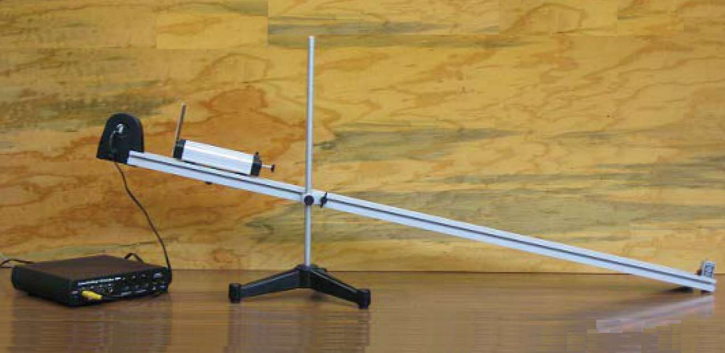
\includegraphics[width=0.5\textwidth]{Rampa_Exp1.png}
        \caption{Configuración del primer experimento}
    \end{figure}

    Considerando que la fuerza de fricción entre el carro y el riel es despreciable, el diagrama de cuerpo libre es el siguiente: 

    \begin{figure}[ht]
        \centering
        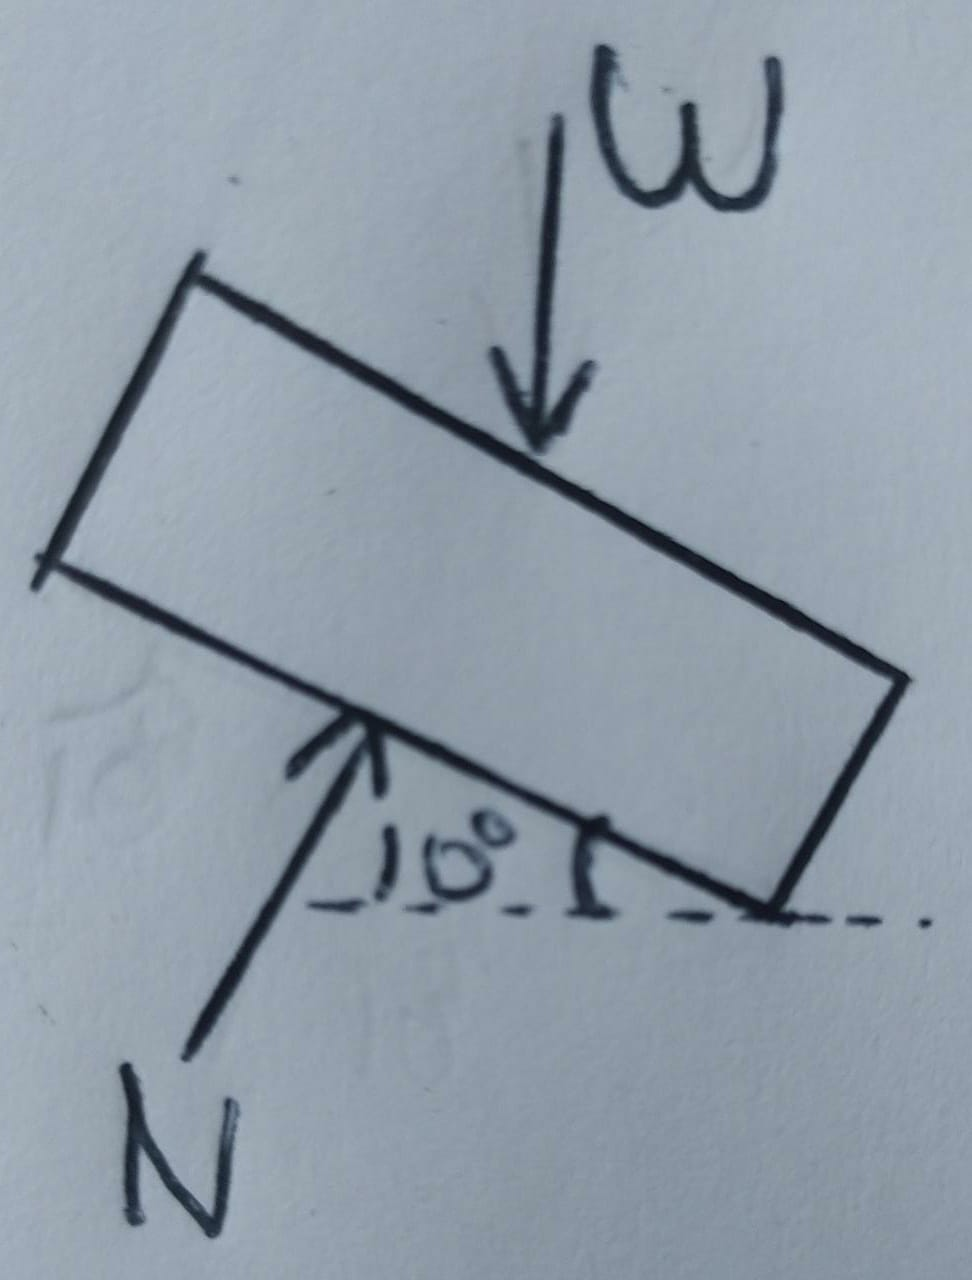
\includegraphics[width=0.15\textwidth]{DCL_E1.jpg}
        \caption{DCL del carro dinámico}
    \end{figure}

    Bajo estas condiciones, su aceleración se puede calcular con la expresión $a=g\sen\theta$, donde $g=9.78[m/s^2]$ y $\theta$ es el ángulo del plano inclinado.
    $$a=9.78\sen(10^\circ) = 1.70[m/s^2]$$

    Para registrar los datos por medio del software \textit{PASCO Capstone} fue necesario configurar el sensor de movimiento: la frecuencia de muestreo se cambió a 50 Hz y el tipo de registro se configuró en basado en tiempo con una duración de 2 segundos. 

    Para la toma de datos fue necesaria la sincronización de por lo menos tres miembros de la brigada. Un miembro se encargó de presionar el botón de \textit{Registro} en la PC, otro miembro sostenía al carro en la posición inicial y un tercer miembro se colocó al final de la rampa para prevenir que el carro se dañara.

    Tras cada medición se exportaron los datos en una memoria USB en formato de texto plano (.txt). Los datos obtenidos tienen el siguiente formato:

    \begin{figure}[ht]
        \centering
        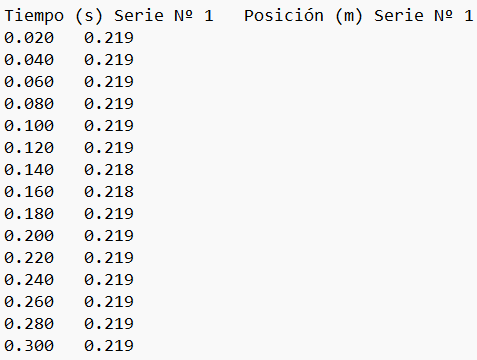
\includegraphics[width=0.5\textwidth]{Formato_Datos.png}
        \caption{Registro de datos}
    \end{figure}
    
    En cada archivo guardado es necesario eliminar los datos iniciales anteriores al inicio del movimiento del carro. Asimismo, se eliminan los datos finales en los que la posición empieza a disminuir o a mantenerse constante.
    
    Una vez eliminados todos los datos que cumplen las condiciones anteriores, se inicia el procesamiento de datos con el software \textit{Mathematica}. El procedimiento siguiente se aplicó a cada archivo de datos:
    
    \begin{enumerate}[a), topsep=0.5cm]
        \item Importar el archivo de datos:
        
        \centerline{\textbf{Datos = Import}[``\textit{dirección del arvhivo}'', ``Data'']}
        \item Crear una variable con el numero de pareja de datos: 
        
        \centerline{\textbf{NumDat = Lenght[Datos]}}
        \item Trasladar los puntos de la variable \textbf{Datos} al origen de la gráfica:
    
        \centerline{\textbf{DatAj = Table[Datos[[$n$]] - Datos[[1]], \{$n$, 1, NumDat, 1\}]}}
        \item Dibujar la gráfica con los datos de \textbf{DatAj}:
        
        \centerline{\textbf{Graf1 = ListPlot[DatAj]}}
        \item Crear un polinomio cuadrático que se ajuste a los datos experimentales: 
        
        \centerline{\textbf{FunX = Fit[DatAj, \{1, $t$, $t^2$\}, $t$]}}
        \item Dibujar la gráfica del polinomio cuadrático: 
        
        \centerline{\textbf{Graf2 = Plot[FunX, \{$t$, 0, 0.9\}]}}
        \item Mostrar las gráficas \textbf{Graf1} y \textbf{Graf2} superpuestas:
        
        \centerline{\textbf{Show[Graf1, Graf2]}}
        \item Obtener los valores de aceleración (\textbf{a}), rapidez inicial (\textbf{b}) y posición inicial (\textbf{c}) a partir del polinomio cuadrático:
        
        \centerline{\textbf{c = FunX /. $t \rightarrow$ 0}}
        \centerline{\textbf{FunV = D[FunX, $t$]}}
        \centerline{\textbf{b = FunV /. $t \rightarrow$ 0}}
        \centerline{\textbf{a = D[FunV, $t$]}}
        \item Copiar los valores de tiempo de la tabla \textbf{DatAj} y evaluarlos en el polinomio cuadrático:
        
        \centerline{\textbf{tExp = Table[DatAj[[n]][[1]], \{$n$, 1, NumDat, 1\}]}}
        \centerline{\textbf{FunXt = Table[FunX /. $t \rightarrow$ tExp[[n]], \{$n$, 1, NumDat, 1\}]}}
        \item Copiar los valores de posición de la tabla \textbf{DatAj}:
        
        \centerline{\textbf{xExp = Table[DatAj[[n]][[2]], \{$n$, 1, NumDat, 1\}]}}
        \item Calcular el error medio cuadrático (\textit{\textbf{rms}} por sus siglas en ingles), comparando los datos experimentales con los del polinomio cuadrático con la siguiente expresión matemática:
        $$e_{rms}=\sqrt{\frac{1}{NumDat} \sum_{i=1}^{NumDat}(FunX(t_i)-xExp(t_i))^2}$$
    \end{enumerate}

    Los conjuntos de datos ajustados (\textbf{DatAj}) de cada toma de datos son los siguientes:

    \begin{longtable}{|c|c|c|c|c|c|}
        \hline
        \# Medición $\rightarrow$ & 1 & 2 & 3 & 4 & 5 \\ \hline
        Tiempo [s] & \multicolumn{5}{c|}{Posición [m]} \\ \hline
        0 & 0 & 0 & 0 & 0 & 0 \\ \hline
        0.02 & 0.001 & 0.001 & 0.001 & 0.002 & 0.001 \\ \hline
        0.04 & 0.002 & 0.003 & 0.002 & 0.004 & 0.002 \\ \hline
        0.06 & 0.005 & 0.005 & 0.003 & 0.006 & 0.003 \\ \hline
        0.08 & 0.007 & 0.008 & 0.006 & 0.01 & 0.005 \\ \hline
        0.1 & 0.011 & 0.012 & 0.009 & 0.014 & 0.008 \\ \hline
        0.12 & 0.015 & 0.016 & 0.013 & 0.019 & 0.011 \\ \hline
        0.14 & 0.02 & 0.022 & 0.017 & 0.024 & 0.016 \\ \hline
        0.16 & 0.026 & 0.027 & 0.022 & 0.03 & 0.02 \\ \hline
        0.18 & 0.032 & 0.034 & 0.028 & 0.037 & 0.026 \\ \hline
        0.2 & 0.039 & 0.042 & 0.035 & 0.045 & 0.032 \\ \hline
        0.22 & 0.047 & 0.05 & 0.043 & 0.053 & 0.04 \\ \hline
        0.24 & 0.056 & 0.058 & 0.05 & 0.062 & 0.047 \\ \hline
        0.26 & 0.065 & 0.068 & 0.059 & 0.072 & 0.056 \\ \hline
        0.28 & 0.075 & 0.078 & 0.069 & 0.082 & 0.065 \\ \hline
        0.3 & 0.085 & 0.089 & 0.079 & 0.093 & 0.075 \\ \hline
        0.32 & 0.097 & 0.1 & 0.089 & 0.105 & 0.085 \\ \hline
        0.34 & 0.109 & 0.112 & 0.101 & 0.117 & 0.096 \\ \hline
        0.36 & 0.121 & 0.125 & 0.112 & 0.129 & 0.107 \\ \hline
        0.38 & 0.134 & 0.137 & 0.125 & 0.143 & 0.119 \\ \hline
        0.4 & 0.149 & 0.154 & 0.138 & 0.157 & 0.132 \\ \hline
        0.42 & 0.161 & 0.166 & 0.153 & 0.172 & 0.146 \\ \hline
        0.44 & 0.177 & 0.182 & 0.168 & 0.188 & 0.162 \\ \hline
        0.46 & 0.193 & 0.199 & 0.184 & 0.205 & 0.177 \\ \hline
        0.48 & 0.21 & 0.216 & 0.2 & 0.222 & 0.193 \\ \hline
        0.5 & 0.227 & 0.233 & 0.218 & 0.241 & 0.21 \\ \hline
        0.52 & 0.246 & 0.252 & 0.236 & 0.26 & 0.228 \\ \hline
        0.54 & 0.265 & 0.271 & 0.254 & 0.279 & 0.246 \\ \hline
        0.56 & 0.285 & 0.291 & 0.274 & 0.299 & 0.265 \\ \hline
        0.58 & 0.304 & 0.312 & 0.294 & 0.32 & 0.285 \\ \hline
        0.6 & 0.325 & 0.333 & 0.314 & 0.342 & 0.305 \\ \hline
        0.62 & 0.347 & 0.355 & 0.336 & 0.364 & 0.327 \\ \hline
        0.64 & 0.369 & 0.378 & 0.358 & 0.387 & 0.348 \\ \hline
        0.66 & 0.392 & 0.401 & 0.381 & 0.411 & 0.371 \\ \hline
        0.68 & 0.416 & 0.425 & 0.404 & 0.435 & 0.394 \\ \hline
        0.7 & 0.44 & 0.449 & 0.428 & 0.46 & 0.418 \\ \hline
        0.72 & 0.465 & 0.475 & 0.453 & 0.486 & 0.442 \\ \hline
        0.74 & 0.493 & 0.501 & 0.478 & 0.512 & 0.467 \\ \hline
        0.76 & 0.517 & 0.528 & 0.505 & 0.539 & 0.493 \\ \hline
        0.78 & 0.544 & 0.555 & 0.532 & 0.567 & 0.52 \\ \hline
        0.8 & 0.574 & 0.583 & 0.559 & 0.596 & 0.547 \\ \hline
        0.82 & 0.602 & 0.612 & 0.588 & 0.625 & 0.575 \\ \hline
        0.84 & 0.631 & 0.641 & 0.617 & 0.654 & 0.604 \\ \hline
        0.86 & 0.659 & 0.671 & 0.646 & 0.685 & 0.633 \\ \hline
        0.88 & 0.689 & 0.702 & 0.677 & 0.717 & 0.663 \\ \hline
        0.9 & 0.721 & 0.734 & 0.708 & - & 0.694 \\ \hline
        0.92 & - & - & - & - & 0.726 \\ \hline
        \caption{Datos ajustados}
    \end{longtable}

    Los ajustes al polinomio cuadrático (\textbf{FunX}) son los siguientes:

    \begin{longtable}{|c|c|}
        \hline
        \# Medición & Ecuación [$m$] \\ \hline
        1 & $7.74746\times10^{-6} + 0.0236804 t + 0.864585 t^2$ \\ \hline
        2 & $0.0000131822 + 0.0334031 t + 0.869083 t^2$ \\ \hline
        3 & $0.00056753 - 0.00483174 t + 0.879114 t^2$ \\ \hline
        4 & $0.000939254 + 0.0417374 t + 0.876859 t^2$ \\ \hline
        5 & $0.00106774 - 0.0205133 t + 0.87869 t^2$ \\ \hline
        \caption{Polinomios cuadráticos}
    \end{longtable}

    \newpage
    Las gráficas superpuestas de \textbf{DatAj} y \textbf{Funx} obtenidas para cada medición se muestran a continuación:

    \begin{figure}[ht]
        \centering
        \begin{minipage}[c]{0.45\linewidth}
            \centering
            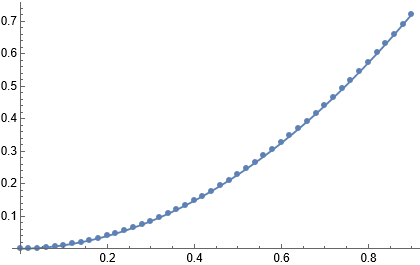
\includegraphics[width=7cm]{Graf1.png}
            \caption{Medición 1}
        \end{minipage} \hspace{.75cm}
        \begin{minipage}[c]{0.45\linewidth}
            \centering
            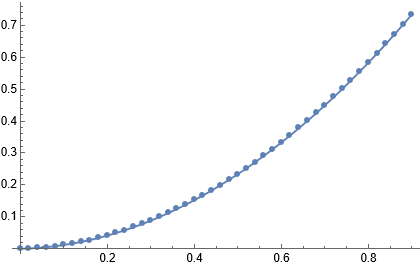
\includegraphics[width=7cm]{Graf2.png}
            \caption{Medición 2}
        \end{minipage}
        \par\bigskip
        \begin{minipage}[c]{0.45\linewidth}
            \centering
            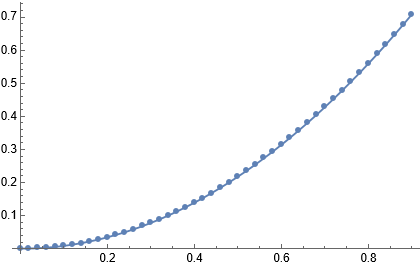
\includegraphics[width=7cm]{Graf3.png}
            \caption{Medición 3}
        \end{minipage} \hspace{.75cm}
        \begin{minipage}[c]{0.45\linewidth}
            \centering
            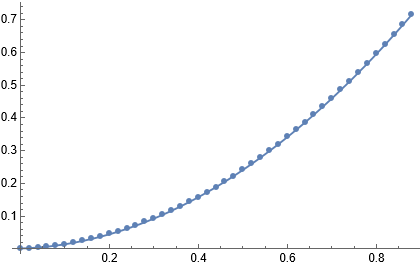
\includegraphics[width=7cm]{Graf4.png}
            \caption{Medición 4}
        \end{minipage}
        \par\bigskip
        \begin{minipage}[c]{0.45\linewidth}
            \centering
            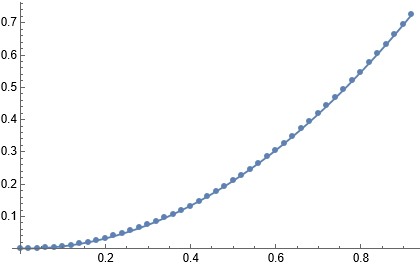
\includegraphics[width=7cm]{Graf5.png}
            \caption{Medición 5}
        \end{minipage}
    \end{figure}
    
    \newpage Los valores de \textbf{a}, \textbf{b}, \textbf{c} y de \textit{\textbf{rms}} obtenidos para cada medición están registrados en la siguiente tabla:

    \begin{table}[ht]
        \centering
        \begin{tabular}{|c|c|c|c|c|}
            \hline
            \multirowcell{2}{\#Medición} & \multirowcell{2}{Aceleración\\inicial [$m/s^2$]} & \multirowcell{2}{Rapidez\\inicial [$m/s$]} & \multirowcell{2}{Posición\\inicial [m]} & \multirowcell{2}{Error medio\\cuadrático} \\
            ~ & ~ & ~ & ~ & ~ \\ \hline
            1 & 1.72917 & 0.0236804 & $7.74746\times10^{-6}$ & 0.000723798 \\ \hline
            2 & 1.73817 & 0.0334031 & 0.0000131822 & 0.000537635 \\ \hline
            3 & 1.75823 & -0.00483174 & 0.00056753 & 0.000475671 \\ \hline
            4 & 1.75372 & 0.0417374 & 0.000939254 & 0.000525488 \\ \hline
            5 & 1.75738 & -0.0205133 & 0.00106774 & 0.000570782 \\ \hline
        \end{tabular}
        \caption[short]{Valores dinámicos}
    \end{table}

    \begin{enumerate}[a), topsep=0.5cm, resume]
        \item Descartar dos conjuntos de datos que tengan el máximo y mínimo valor de error medio cuadrático. Eliminaremos las mediciones 1 y 3. 
        \item Calcular el promedio de los valores de \textbf{a}, \textbf{b} y \textbf{c}:
        
        \centerline{\textbf{aProm = Mean[\{a2, a4, a5\}]} = 1.74975}
        \centerline{\textbf{bProm = Mean[\{b2, b4, b5\}]} = 0.0182091}
        \centerline{\textbf{cProm = Mean[\{c2, c4, c5\}]} = 0.000673391}

        \item Establecer la función de posición que representa a todo el experimento:
        
        \centerline{\textbf{FunXprom =  $\frac{1}{2}$ aProm$t^2$ + bProm$t$ + cProm}}
        \centerline{$0.000673391 + 0.0182091 t + 0.874877 t^2$ [$m$]}

        \item Dibujar la gráfica de rapidez, \textbf{FunVprom} vs. tiempo, derivando a la función \textbf{FunXprom}:
        
        \centerline{\textbf{FunVprom = D[FunXprom, $t$]}}
        \centerline{$0.0182091 + 1.74975 t$ [$m/s$]}
        \centerline{\textbf{Plot[[FunVprom], \{$t$, 0, 0.7\}]}}

        \begin{figure}[ht]
            \centering
            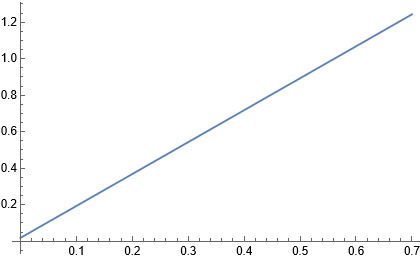
\includegraphics[width=0.45\textwidth]{Graf_Rapidez.png}
            \caption{Gráfica de la rapidez promedio}
        \end{figure}

        \newpage
        \item Obtener la gráfica de aceleración, \textbf{AcelProm} vs. tiempo, que se obtiene derivando la función \textbf{FunVprom}:
        
        \centerline{\textbf{Acelprom = D[FunVprom, $t$]}}
        \centerline{$1.74975$ [$m/s^2$]} 
        \centerline{\textbf{Plot[[Acelprom], \{$t$, 0, 0.7\}]}}

        \begin{figure}[ht]
            \centering
            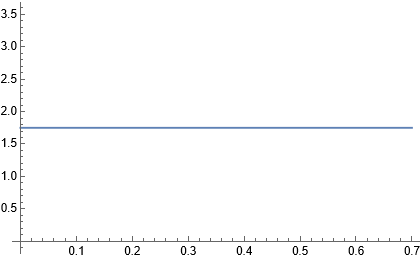
\includegraphics[width=0.45\textwidth]{Graf_Aceleracion.png}
            \caption{Gráfica de la aceleración promedio}
        \end{figure}

        \item Establecer una ecuación de \textbf{FunVprom} igualado o la variable \textbf{Vel}, y despejar la variable tiempo:
        
        \centerline{\textbf{ecuación1 = FunVprom == Vel}}
        \centerline{\textbf{solución1 = Solve[ecuación1, $t$]}}
        \centerline{\textbf{tSol = $t$ /. solución1[[1]]}}

        \item Sustuir tSol en lugar de la variable tiempo en la ecuación de \textbf{FunXprom} igualando \textbf{X}, y obtener \textbf{Vel} en función de \textbf{X}:
        
        \centerline{\textbf{ecuación2 = (FunXprom /. $t\rightarrow$ tSol) == X}}
        \centerline{\textbf{solución2 = Solve[ecuación2, $t$]}}
        \centerline{\textbf{VelSol = Vel /. solución2[[2]]}}

        \item Dibuje la gráfica de la expresión de la rapidez, \textbf{Vel}, en función
        de la posición, \textbf{X}, la cual se conoce como “plano de fase”:

        \centerline{\textbf{Plot[[VelSol], \{X, 0, 0.85\}]}}

        \begin{figure}[ht]
            \centering
            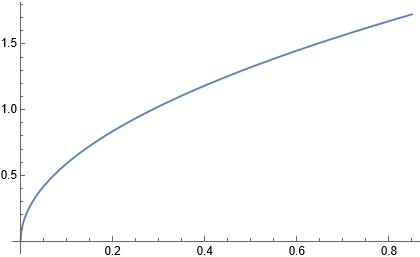
\includegraphics[width=0.45\textwidth]{Plano_de_Fase.png}
            \caption{Plano de Fase}
        \end{figure}
    \end{enumerate}

    \newpage
    Para finalizar con el primer experimento se compararan los valores de aceleración ``teóricos'' y ``experimentales''. El valor de la aceleración teórica fue de 1.70 [$m/s^2$] y el valor de la aceleración experimental fue de 1.74975 [$m/s^2$]. Con estos datos es posible calcular el porcentaje de error experimental:
    $$\%EE=\frac{|Aceleracion_{teorica}-Aceleracion_{experimental}|}{Aceleracion_{teorica}}\times100\%$$
    $$\%EE=\frac{|1.70-1.74975|}{1.70}\times100\%=2.93\%$$

    Con un porcentaje de error relativamente bajo de aproximadamente 3\% demuestra que el experimento se realizó siguiendo correctamente las instrucciones, asimismo, demuestra que la manera teórica de calcular la aceleración es comprobable. Que el error no haya sido del 0\% se puede deberse a causas como una ligera variación o interferencia en la realización de las mediciones o de un redondeo de decimales en los cálculos.

    \section*{Segundo Experimento}
    El experimento consiste en estudiar el movimiento de un carro sobre un riel de aire. Se ajusta el riel en un ángulo de 12° con respecto a la horizontal y se tapan los orificios. Se coloca un contenedor boca abajo cerca del extremo más alto del riel y se colocan dos compuertas optoelectrónicas a diferentes distancias. Luego, se suelta el carro cerca de la primera compuerta y se enciende la compresora de aire. 
    
    El cronómetro registra el tiempo mientras el carro adquiere velocidad y luego se desacelera hasta detenerse. Se toman varias mediciones de distancia, tiempo y altura para estimar el ángulo del riel con respecto a la horizontal. El experimento se repite varias veces para obtener resultados más precisos.

    \begin{figure}[ht]
        \centering
        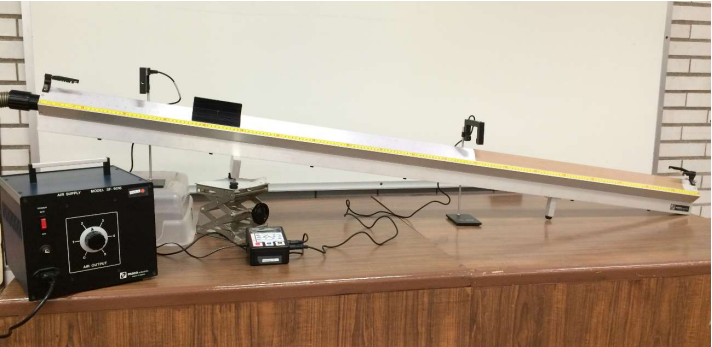
\includegraphics[width=0.5\textwidth]{Rampa_Exp2.png}
        \caption{Configuración del segundo experimento}
    \end{figure}
    
    Considerando que en esta parte del riel, la fuerza de fricción entre el carro y el riel es despreciable, el diagrama de cuerpo libre es el siguiente:

    \begin{figure}[ht]
        \centering
        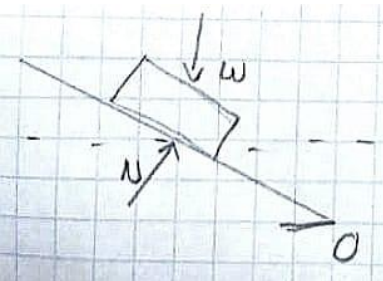
\includegraphics[width=0.5\textwidth]{DCL_E2.png}
        \caption{DCL del carro para riel de aire}
    \end{figure}

    Con base en el diagrama de cuerpo libre, se pueden establecer las expresiones para la aceleración, constante, así como la rapidez y la posición en función del tiempo y del ángulo de inclinación.

    Para sin fricción:
    $$\sum F_x = W\sen\theta = ma$$
    $$\sum F_y = N - W\cos\theta = 0$$

    Usamos $a = g\sen\theta$ de $v = v_0 y v_0t + \frac{1}{2}at^2$
    $$x = \frac{1}{2}at^2 \Rightarrow a = \frac{2x}{t^2}$$

    A partir de las expresiones anteriores, se calculó el ángulo de inclinación del riel, con base en la distancia entre las compuertas optoelectrónicas medida durante la realización del experimento y el tiempo promedio de los medidos con el cronómetro digital, considerando que la aceleración de la gravedad es $g = 9.78$ [$m/s^2$]

    Distancia entre compuertas = 80 [$cm$]

    \begin{longtable}{|c|c|c|}
        \hline
        \multirowcell{2}{Medición} & \multirowcell{2}{Tiempo registrado entre\\las compuertas [$s$]} & \multirowcell{2}{Distancia recorrida en la\\cinta canela [$m$]} \\
        ~ & ~ & ~ \\ \hline
        1 & 0.8265 & 47.5 \\ \hline
        2 & 0.8467 & 47.4 \\ \hline
        3 & 0.8361 & 47.8 \\ \hline
        4 & 0.8404 & 55 \\ \hline
        5 & 0.8396 & 50 \\ \hline
    \end{longtable}
    \newpage
    
    \centerline{$F = 0.83803$ [$N$]}
    \centerline{$v = 0.79$ [$m/s$]}
    \centerline{$a = \frac{2(0.79)}{(0.83803)^2} = 2.2497$ [$m/s^2$]}

    Sustituimos en $a = g\sen\theta$
    $$2.2497 = 9.78\sen\theta$$

    Despejamos:
    $$\theta = \sen^{-1} (\frac{2.2497}{9.78})$$
    $$\theta = 13.2988^\circ$$

    Con base en las expresiones de posición y velocidad del móvil, así como en el ángulo de inclinación estimado del riel de aire con respecto a la horizontal, obtenido al final del punto 5, y la distancia entre las compuertas optoelectrónicas, es posible determinar la velocidad final en dicho intervalo de movimiento.

    Para rapidez final:
    $$v = v_0 + at$$
    $$v = at$$
    $$v = (2.2497)(0.83803)$$
    \centerline{$v = 1.8853$ [$m/s$]}

    Considerando que la fuerza de fricción cinética de la cinta canela está presente en el carro, el diagrama de cuerpo libre es el siguiente:

    \begin{figure}[ht]
        \centering
        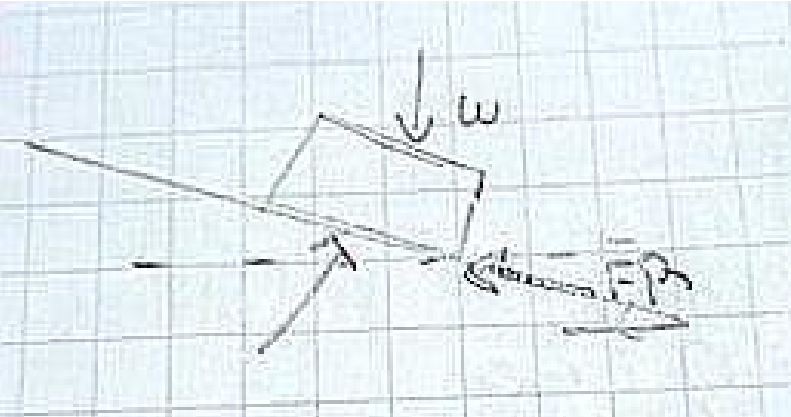
\includegraphics[width=0.45\textwidth]{DCL_E22.png}
        \caption{DCL del carro para riel de aire con fricción presente}
    \end{figure}

    Luego, se establecen las ecuaciones de movimiento del carro en el intervalo anterior, en función del tiempo, considerando el ángulo conocido igual al que se estimó con base en trigonometría, considerando como condición inicial de rapidez, la rapidez final del intervalo de movimiento anterior, calculada anteriormente.
    $$v = 1.88853 [m/s]$$
    $$\theta = 13.2988^\circ$$
    
    Fricción de movimiento: 
    $$\sum F_x = W\sen\theta = ma$$
    $$\sum F_y = N - W\cos\theta = 0$$

    Ocupamos $N$:
    $$N = W\cos\theta$$

    Despejamos:
    $$MK = \frac{ma - W\sen\theta}{-W\cos\theta} \Rightarrow \frac{g\sen\theta - a}{g\cos\theta}$$

    Sustituimos los datos:
    $$MK = \frac{9.78\sen(13.2988) - (-0.019)}{9.78\cos(13.2988)} = 0.23836$$

    Tenemos que:
    $$v^2 = v^2 + 2a(x - x_0)$$

    Despejamos $a$:
    $$a = -\frac{v^2}{2x} = -\frac{(1.8853)^2}{2(49.59)} = 0.019[m/s^2]$$

    Con base en el valor de $g$ mencionado, y la distancia recorrida promedio de las cinco que se midieron durante la realización del experimento, se puede obtener el valor del coeficiente de fricción cinética, $k$, al sustituir los valores de posición y rapidez finales en las expresiones cinemática en este intervalo de movimiento.
    $$\mu = \tan\theta - \frac{a}{g\cos\theta} = 0.2343$$

    \newpage
    \section*{Conclusiones}
    \textbf{Acosta Porcayo Alan Omar:}\\
    La realización de esta práctica fue de utilidad para aplicar los conocimientos sobre cinemática y dinámica que hemos adquirido durante el curso. Los objetivos que se plantearon al principio fueron cumplidos, pues se realizaron los experimentos y los cálculos correspondientes, y también utilizamos herramientas de software para la toma y el procedimiento de mediciones experimentales. 
    
    \textbf{Bonilla López Mauricio Gael:}\\
    Este experimento resultó fácil de hacer, aportando un gran apoyo visual a los temas vistos en clase, junto con el software que se utilizó considero que se lograron los objetivos de la práctica y una mejor comprensión sobre el movimiento y desplazamiento en una superficie inclinada.
    
    \textbf{Cisneros Rojas Héctor Manuel:}\\
    Mediante esta práctica, adquirimos conocimientos sobre cómo determinar la aceleración de un móvil que se desliza hacia abajo en una pendiente inclinada, sin considerar la presencia de fricción. Esta determinación se puede realizar tanto de forma teórica como práctica. Además, logramos el objetivo de utilizar eficazmente el software \textit{Mathematica} como una herramienta para generar gráficas con mayor precisión. Esto nos permitió comprender de manera más profunda los fenómenos mecánicos que estábamos investigando.
    
    \textbf{Domínguez González Andrea:}\\
    La práctica fue muy interesante, porque en el primer experimento pudimos entender con mayor precisión y aplicación en el mundo físico cómo actúa la fuerza de fricción, y en el segundo experimento pude ver (y de una manera muy interesante) cómo la fuerza de rozamiento en el aire (que es bastante ingenioso, algo que nunca se me había ocurrido y desconocía), sin duda podríamos concluir que la fuerza de rozamiento juega un papel importante en el movimiento de objetos.

    \section*{Bibliografía}
    Práctica 5. Movimiento rectilíneo uniformemente variado. Manual de Prácticas del Laboratorio de Mecánica, División de Ciencias Básica, 2022. \url{https://bit.ly/43A70I3}
    
\end{document}